\documentclass[notitlepage]{article}
\usepackage[utf8]{inputenc} 
\usepackage{geometry} 		
\usepackage{chngcntr}
\usepackage{amsmath} 			
\usepackage{amssymb}			
\usepackage{mathtools}		
\usepackage{comment} 			
\usepackage{mdframed}			
\usepackage{xcolor}				
\usepackage{fancyhdr}			
\usepackage{listings}			
\usepackage{color}				
\usepackage{tikz}	
\usepackage{tasks}			
\usepackage{exsheets}	
\usepackage{blindtext}	
\usepackage{array}			
\usepackage{empheq}
\usepackage{caption}
\usepackage{pdfpages}
\usepackage{tabularx}
\usepackage{lscape}

\geometry{ 						%Format titlepage (interrupted by newgeometry)
	a4paper,
	total={170mm,257mm}%,
	%left=0mm,
	%top=0mm,
}

%START DEFINE YOUR VARIABLES HERE

\newcommand{\documentName}{Software Design Specification}
\newcommand{\projectName}{Label Refinement by Behavioral Similarity}

%END DEFINE YOUR VARIABLES HERE

\title{%
	\documentName\text{ } \\
  \large \projectName\text{ } \\
  }

\author{
	\large \underline{Document owners:}\\ 
	Bianka Bakullari\\
	\texttt{}
	Christopher Beine\\
	\texttt{}
	Nicole Ventsch\\
	\texttt{}
	Juan Garza\\
	\texttt{}
}

\date{\small{Last edited: \today}}

\pagestyle{fancy}
\fancyhf{}
\rhead{}
\lhead{\documentName\space-\space\projectName}

\makeatletter					%Prefix to add ToC to titlepage
\newcommand*{\toccontents}{\@starttoc{toc}}
\renewcommand*\contentsname{}
\makeatother
                  

\begin{document}

\begin{titlepage}
\clearpage\maketitle			%Clear title page
\thispagestyle{fancy}
\tableofcontents
\end{titlepage}

\rfoot{\thepage}				%Start printing page-numbers, after title page.

\newgeometry{ 					%Default page formatting on-going #1
	total={170mm,257mm},
	left=20mm,
	top=25mm,
    bottom=30mm					%Causes warning
}

\begin{flushleft}				%Default page formatting on-going #2


\section{Introduction}
\subsection{System Overview}
\subsection{Design Map}
\subsection{Supporting Materials}
\subsection{Definitions and Acronyms}

\section{Design Considerations}
\subsection{Assumptions and Dependencies}
\subsection{General Constraints}
\subsection{Goals and Guidelines}
\subsection{Development Methods}

\section{Architectural Strategies}
{\color{gray} **** under construction ****}
\begin{itemize}
	\item Factory Pattern
	\item Decorator (Variaton)
\end{itemize}

{\color{gray} ***************************}
\section{System Architecture}
\includegraphics[scale=0.4]{"UML_Architecture/Architecture Overview".png}

\subsection{Client Machine}
\subsection{Front-end}
\subsection{Refining Label API}
\subsection{File Store}
\subsection{Refining Event Labels}
\begin{landscape}
\subsection{Event Log Converter}
\includegraphics[width=\columnwidth]{"UML_Architecture/Event Log Converter CD".png}
\end{landscape}
\section{Policies and Tactics}

\section{Detailed System Design}
The main algorithm "Refining Event Labels" will be split up into multiple modules that contain the main parts of the algorithm. These modules will be explained in detail in the following subsections.
\subsection{Module 1: Preprocessing}
Name: Preprocessing

Type: module

Description: This module is responsible for preprocessing the data. The event log provided by the user is read and stored internally. Moreover, it is checked if it has the right format and an error is produced if is does not have. 

Attributes: None

Resources: None

Operations: 
\medskip

\par
\begingroup
\leftskip4em
Name: read\_csv()

Arguments: path to a log file in csv format

Returns: event log 

Description: The csv file provided by the user is read and stored as a table containing the original columns.

Precondition: the path leads to a csv file

Postcondition: the table is stored internally

Exceptions: None
\par
\endgroup

\medskip

\par
\begingroup
\leftskip4em
Name: read\_XES()

Arguments: path to a log file in XES format

Returns: event log 

Description: The XES file provided by the user is read and stored as a table containing the original columns.

Precondition: the path leads to an XES file, the provided column names exist in the file

Postcondition: an event log is stored internally

Exceptions: None
\par
\endgroup

\medskip

\par
\begingroup
\leftskip4em
Name: check\_event\_log()

Arguments: table imported using read\_XES() or read\_csv(),  name of the activity column, ID column and time stamp column provided by the user

Returns: True or False

Description: The table we created by reading in the file is checked for actually being an event log, i.e., containing an activity column, an ID column and a time stamp column. The names for these columns are entered by the user. If these exist in the table, True will be returned, otherwise False will be returned. 

Precondition: a file was read and the names for the columns were entered by the user

Postcondition: the process can continue if True was returned, else an error occurs

Exceptions: None
\par
\endgroup


\subsection{Module 2: Storing the Traces}
Name: Storing the Traces

Type: module

Description: This module is responsible for getting the unique traces from the event log and storing the traces for each activity in a look-up table that can be used for refining the original log later. 

Attributes: None

Resources: None

Operations: 
\medskip

\par
\begingroup
\leftskip4em
Name: create\_lookup\_table()

Arguments: table,  name of the activity column, ID column and time stamp column

Returns: lookup table containing one trace for every ID , where the trace is stored as an array

Description: The table is converted, so that we get the activity traces for each ID ordered by their time stamp.

Precondition: check\_event\_log() returned True

Postcondition: a lookup table is stored

Exceptions: None

\par
\endgroup

\medskip

\par
\begingroup
\leftskip4em
Name: get\_unique\_traces()

Arguments: look-up table created using create\_lookup\_table()

Returns: an array containing the unique traces, i.e., an array of arrays

Description: The traces from the look-up table are checked for duplicates and the unique traces are stored in an array

Precondition: a lookup table was created using create\_lookup\_table()

Postcondition: an array of arrays containing the unique traces is stored

Exceptions: None

\par
\endgroup

\subsection{Module 3}
%...

\section{User Interface Design}
\subsection{Application Control}

In the project, we will implement a web service. The web client will have a rather plain design that should focus on the main activities the service should provide, which are uploading event logs in csv or XES format, setting the threshold for the label refinement algorithm and download the refined log after the algorithm is finished. There will be buttons used to upload the file, apply the algorithm and download the refined event log. Moreover, the screens will have short explanations telling the user what to do (if not self-explanatory). For setting the thresholds, two boxes will be provided that include the default thresholds, but new values can be entered by the user. A draft of each of the main screen can be found in the next section, section 6.2.

\subsection{The Screens}

The main screens will be visualized in the following subsections. In these screens include the main functionalities, which are described in the former section. The following diagram will show the flow of control through the screens.  

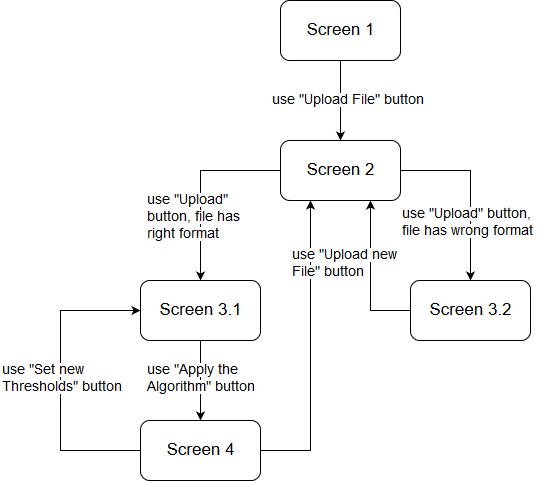
\includegraphics[scale=0.7]{ScreenFlow.png}

\subsubsection{Screen 1}

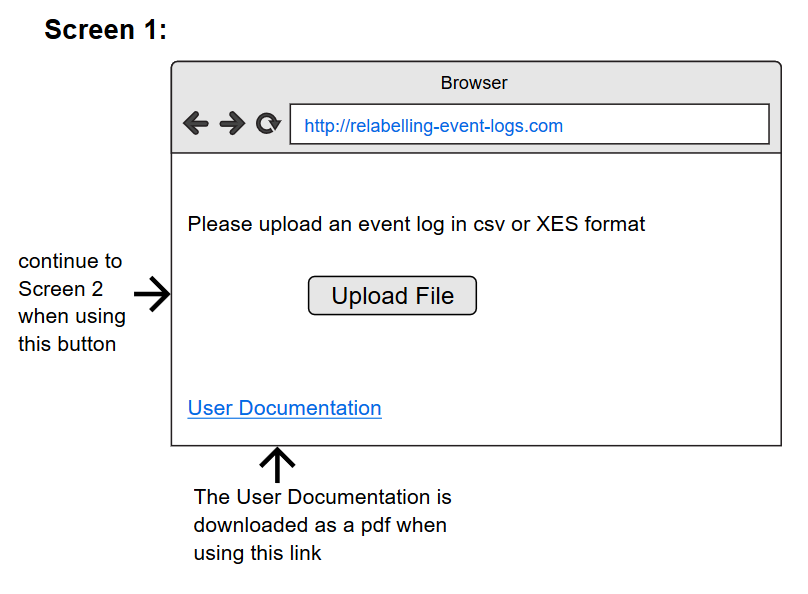
\includegraphics[scale=0.8]{InterfaceMockup1.png}


The first screen visible to the user will show a description saying that an event log in csv of XES format should be uploaded. Moreover, a button "Upload File" is visible. By using this button, the user will continue to Screen 2. At the end of the page, there will be a link called "User Documentation". By clicking on this link, the User Documentation will be downloaded in pdf format.
\subsubsection{Screen 2}

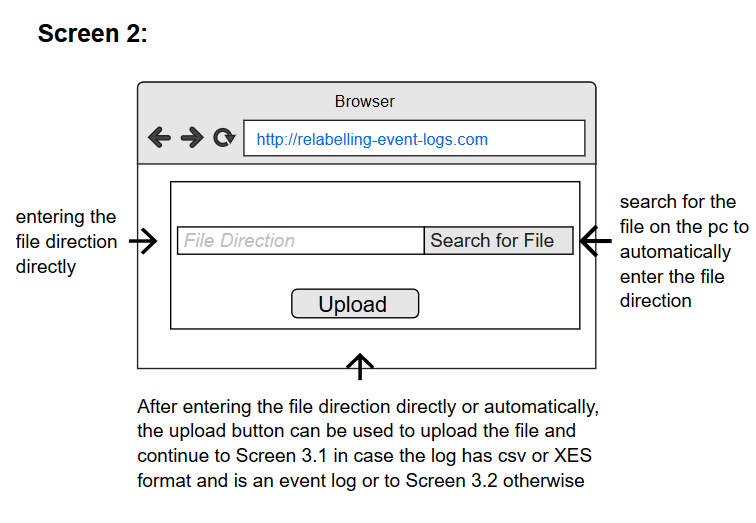
\includegraphics[scale=0.8]{InterfaceMockup2.png}

In the second screen visible to the user, the user can enter the file direction of the event log he wants to upload. He can either directly type in the direction into the "File Direction" field or use the "search for File" button to search for a file on his pc, so that the direction will automatically be filled in after selecting a file.

After using one of this alternatives, he can use the "Upload" button to upload the file with the given directory. In case this file is an event log, i.e., the data contains at least the attributes "id", "time stamp" and "activity name", and has either csv or XES format, the user will continue to Screen 3.1. If one of these conditions is not satisfied, he will continue to Screen 3.2. 


\subsubsection{Screen 3.1}
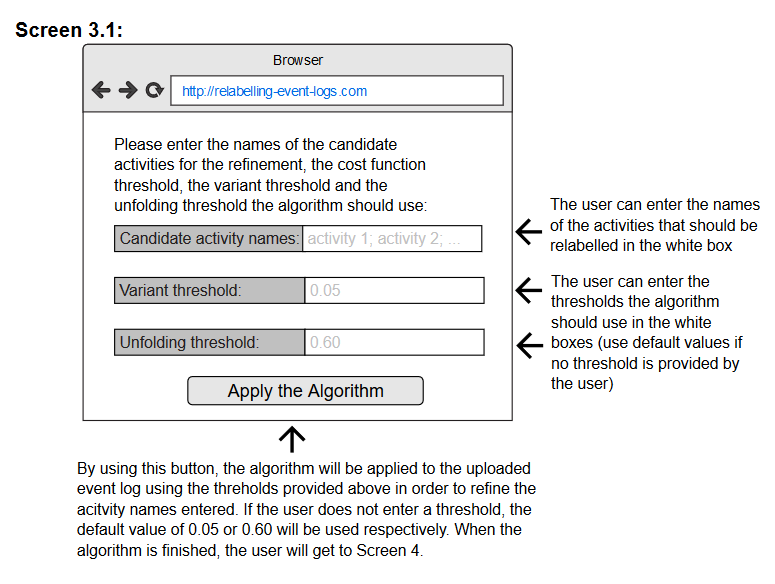
\includegraphics[scale=0.8]{InterfaceMockup3-1.png}

This screen appears if the file uploaded by the user meets the requirements. In this screen, the user can set the thresholds for the algorithm, i.e., the variant and the unfolding threshold. He can enter these in the corresponding white boxes. If he does not enter the thresholds, the default values of 0.05 and 0.60 will be used respectively. Using the button "Apply the Algorithm", the web service will start applying the algorithm using the provided thresholds. After the algorithm is finished, the user will get to Screen 4.

\subsubsection{Screen 3.2}
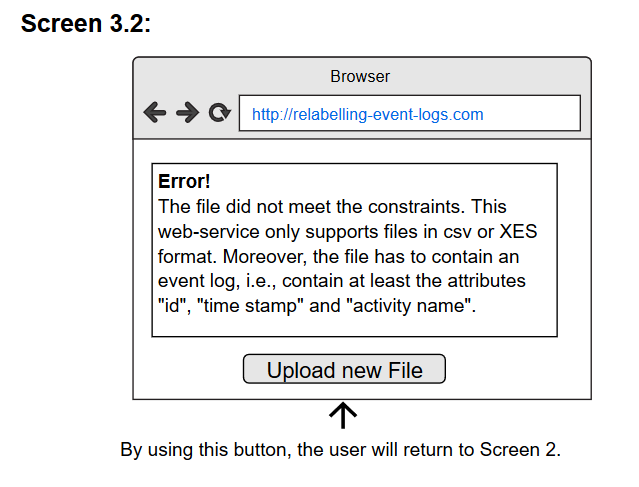
\includegraphics[scale=0.8]{InterfaceMockup3-2.png}

This screen appears if the upload was not successful because the file did not meet the assumptions. If the file does not have the right format, the user can click on the button "Upload new File" to return to Screen 2 and upload a file that meets the constraints.


\subsubsection{Screen 4}
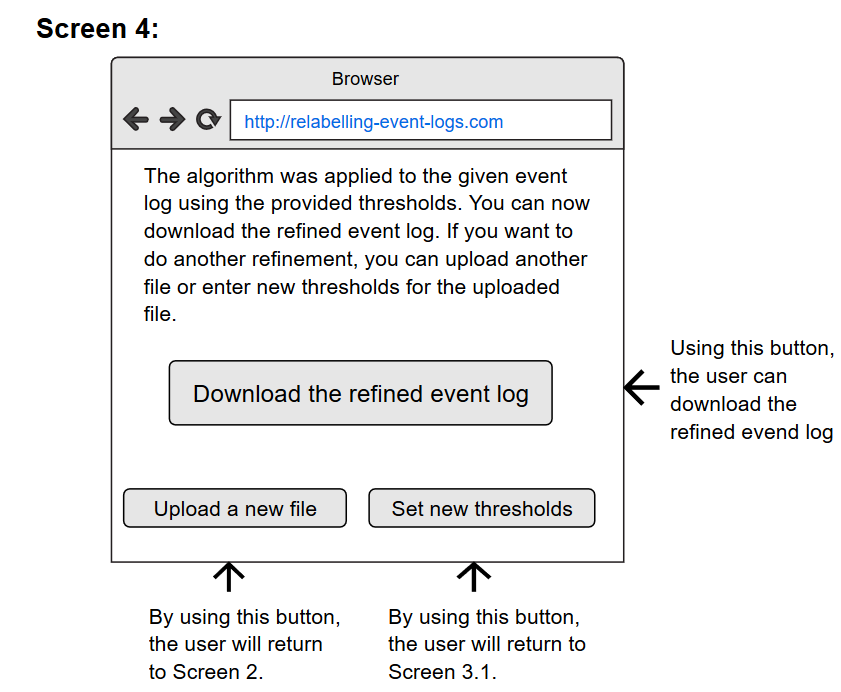
\includegraphics[scale=0.8]{InterfaceMockup4.png}

This Screen will be shown after finishing the algorithm. The user can now download the refined log using the corresponding button. After this step, the user is done and can exit the page, but if he also wants to apply the algorithm to another event log or to the same event log using different thresholds, he can use the corresponding buttons and will be redirected to Screen 2 or Screen 3.1 respectively.


%\newpage
%\bibliographystyle{plain}
%\bibliography{references}  




%\addcontentsline{toc}{chapter}{\textbf{References}}
\end{flushleft}
%\bibliography{uw-ethesis}
% Tip 5: You can create multiple .bib files to organize your references. 
% Just list them all in the \bibliogaphy command, separated by commas (no spaces).

% The following statement causes the specified references to be added to the bibliography% even if they were not 
% cited in the text. The asterisk is a wildcard that causes all entries in the bibliographic database to be included (optional).


\begin{thebibliography}{5}
\bibitem{paper}
Lu, Xixi, et al. "Handling duplicated tasks in process discovery by refining event labels." International Conference on Business Process Management. Springer, Cham, 2016.




\end{thebibliography}










\end{document}
